\chapter{Cognitive theories}

\label{ch:theory}

This chapter aims to explain the effectivity and inner workings of both concept mapping and flashcard systems by elaborating on the physiology of the relevant parts of the brain and the relevant cognitive theories, since these provide relevant information for the design of the flashcard and flashmap system. However, a general overview of the types of learning will be addressed, and the type of learning involved within this project, in order to provide focus on the specific cognitive theories relevant for the software design.

\section{Types of learning}

According to \citeA{squire}, there are multiple varieties of memory, which can mainly be categorised into declarative and nondeclarative knowledge, sometimes also referred to as respectively explicit and implicit knowledge \cite{cognitivepsychology}. Declarative knowledge also refers to memories that can be explicitly recalled, entailing facts such as definitions, paired associations etc., but also the events where these facts were acquired. Nondeclarative memory involves every memory which can be demonstrated in action, but not in conscious recall per se. Subcategories of these memories are procedural skills, priming, conditioning, and nonassociative memories. Because of the nature of this study, the cognitive theories discussed below are mainly focused on declarative knowledge, although most theories also are relevant to nondeclarative memory in some degree.

Furthermore, \citeA{instructionaldesign} describes declarative knowledge as one of Gagné's types of learning outcomes, and relates declarative knowledge to Bloom's levels of recall and understanding, meaning that declarative knowledge does not only encompass rote memorisation of facts, but also understanding the meaning behind this fact. This is also in line with the essay written by \citeA{glaserfield} on radical constructivism, in which it is stated that whatever it is that students are to place into memory they should also understand. Another category of learning outcomes applicable to this context is that of intellectual skills, mainly that of concepts. These, according to \citeA{instructionaldesign}, help the learners simplify the world and can make them into more efficient thinkers. From a cognitive perspective however, there is not a great difference in dealing with declarative knowledge or concepts, because both relate to explicitly recallable memories and thereby can both be considered as being explicit \cite{squire}.

\section{Storage and retrieval}

\begin{figure}
    \centering
    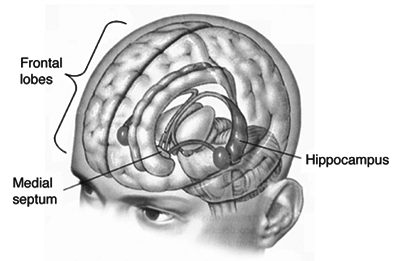
\includegraphics[width=0.5\textwidth]{img/brainareas.png}
    \caption{The brain areas mainly involved in storing and retrieving declarative knowledge \protect\cite{amnesia}}
    \label{fig:brainareas}
\end{figure}

Although the whole brain is involved in storing memories, the most prominent areas facilitating the process of memorising are the frontal lobes and the hippocampus \cite{cognitivepsychology} (see figure~\ref{fig:brainareas}). The prefrontal regions are responsible for the creation and retrieval of memories, whereas the hippocampal and surrounding areas allow permanent storage of these memories. Because of this dynamic, \citeA{modalmemory} conceived a modal theory of memory, displayed in figure~\ref{fig:modalmemory}. In this model, information is perceived as sensory input, and is then shortly stored in the sensory memory. If the perceiver has paid enough attention to the input, it is then transfered (or encoded) into short-term memory. When the input is strong enough, that is, rehearsed often enough within short term memory, it can be more permanently stored in long-term memory. If not, the input fades away from memory and is forgotten. When a memory exists in long-term memory, it has to be retrieved into short-term memory in order to be remembered and used.

\begin{figure}
    \centering
    
\includegraphics[width=0.5\textwidth]{img/modalmemory.png}
    \caption{The modal model of memory proposed by \protect\citeA{modalmemory}}
    \label{fig:modalmemory}
\end{figure}

\citeA{karpicke4} describes two seperate learning practices based on the modal model of memory, namely encoding and retrieval practices, where encoding practices are focused on meaningful encoding or construction of knowledge, and retrieval practices are more focused on the reconstruction and rehearsal of knowledge. He states that both practices are essential to enhancing learning. The flashcard systems described in the \nameref{sec:intro_fc} on page~\pageref{sec:intro_fc} are a famous retrieval practice, which emphasise drilling the same pairs by association over and over again. Concept maps, described in the \nameref{sec:intro_cmap} on page~\pageref{sec:intro_cmap} are often regarded as a encoding practice, since the student has to connect diverse concepts within one topic by meaningful relations.

The following sections will elaborate on cognitive effects with regard to both encoding and retrieval practices, and relating them with their relevance to the effectiveness of concept mapping and flashcard systems respectively.

\section{Cognitive effects with regard to encoding practices}

\subsection{The brain as an associative network}

The brain is structured as an associative network, where neurons function as nodes, and synapses function as edges. When something has to be retrieved from memory, neurons signal relevant neighbouring neurons through the synapses in order to activate the relevant parts of the brain. More generally speaking, when stimulated with a retrieval cue, the brain can then use neural pathways to find a corresponding item in the brain. These networks are sometimes referred to as \emph{semantic networks}, and the implication for retrieval as \emph{spreading activation} \cite{cognitivepsychology}. This effect has also been found on a cognitive level, for example \citeA{kintsch} has found that material is often not literally encoded, but rather as a set of abstract meaning units representing certain associations between concepts.

\subsection{Elaborative processing}

Because information is retrieved in the brain via related nodes and edges in the semantic network, strong neural pathways facilitate the retrieval process. One way of creating these pathways is elaborative processing \cite{karpicke4, cognitivepsychology}, which focuses on meaningful processing of the content. \citeA{craik} conducted an experiment where students were to freely recall from a list of words after the students had to train the words by one of the following techniques: answering questions about structural details (e.g. is it in capital letters); about phonemical details (e.g. the word rhyming on another word); whether the word fits into a certain category; and whether the word fits in a certain sentence. They found that the more meaningful the task was, the higher the retrieval rate was, which was later confirmed by \citeA{barclay}. Furthermore, research conducted by \citeA{nelson} presented students with paired associates that where either semantic or phonetic (in this case rhymes), and students showed a significantly higher recall of semantic associates. These studies demonstrate the importance of meaningful processing for retention.

\subsection{Implications for concept mapping}

Reflecting on the previously described theory of associated networks, it appears that a semantic network is very similar in structure to concept maps, and thereby the maps provide an accurate representation of the way information is retrieved from the brain. For example, \citeA{canas} states that "the widespread use of concept maps is based on the notion that a concept map is a reflection of the builder's cognitive structure and thus portrays his or her understanding of the domain depicted in the map" (p. 1). \citeA{nesbit} speculate that because of this, more and better retrieval cues are created when learning from or generating a concept map. Furthermore, a concept map highlights the meaningful relations between the concepts, rather than just teaching the concepts themselves.

\section{Cognitive effects with regard to retrieval practices}

According to \citeA{karpicke4}, a lot of educational practices have placed an emphasis on finding optimal ways to encode knowledge and experiences, but that retrieval practices have received less attention. Nevertheless, basic research has indicated that retrieval is still important to consider in any analysis of learning. This is mainly due to the fact that information is not stored exactly and indefinitely, but rather that memories are forgotten over time. Two theories explaining why forgetting occurs have been proposed and debated over, namely it occuring because of interference by other redundant memories, and it occuring because of decay of existing memories. Although both the effect of interference and decay have been proposed as separate theories and have been debated, they are not mutually exclusive, and \citeA{cognitivepsychology} therefore conludes that forgetting results both from decay and from interference.

\subsection{Power laws of forgetting and learning}

When designing for memory retention, it is important to investigate with which rate people learn and forget. Already in 1885, Ebbinghaus discovered the power law of learning, referred to as the inversal exponential nature of forgetting \cite{microlearning, activationbasedmodel}. The implication of this model is that memory not only systematically deteriorates with delay, but also that this loss is negatively accelerated, meaning that the rate of change gets smaller with increasing delay \cite{cognitivepsychology}. \citeA{wickelgren} already proposed the formula $m = \lambda (1 + \beta t)^{-\psi}$, where $m$ is memory strength (the probability of recognition), $t$ is time, $\lambda$ is the state of long-term memory at $t = 0$, $\psi$ is the rate of forgetting, and $\beta$ is the scaling parameter (see figure~\ref{fig:powerlawforgetting}). This formula has also found to be accurate by \citeA{wixted}. 

\begin{figure}
    \centering
    \begin{subfigure}{0.7\textwidth}
        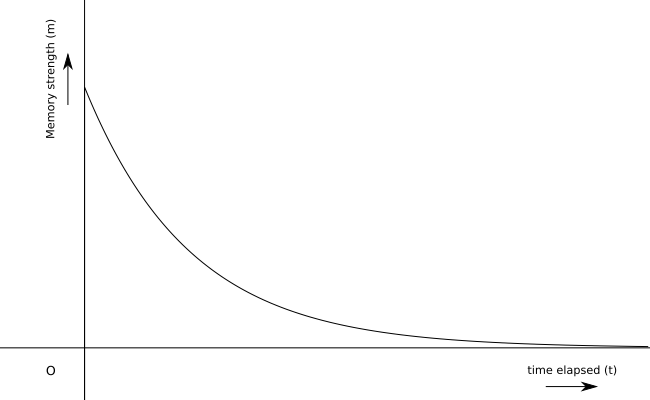
\includegraphics[width=\textwidth]{img/powerlawforgetting}
        \caption{The power law of forgetting, with m as the probability of recognition and t as the time passed since learning}
        \label{fig:powerlawforgetting}
    \end{subfigure}
    \par\bigskip
    \begin{subfigure}{0.7\textwidth}
        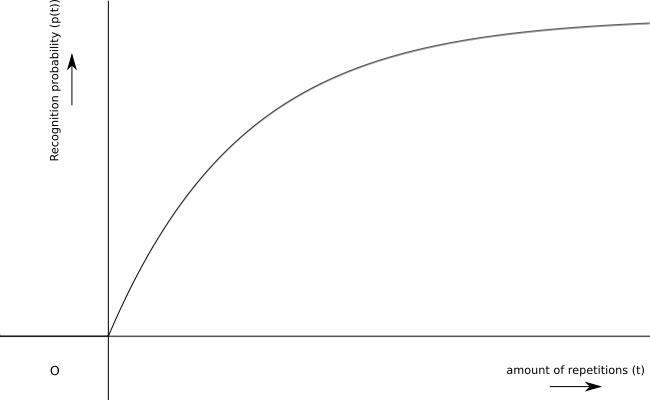
\includegraphics[width=\textwidth]{img/powerlawlearning}
        \caption{The power law of forgetting, with p(t) as the probability of recognition and t as the iterations of learning}
        \label{fig:powerlawlearning}
    \end{subfigure}
    \caption{The power laws of learning and forgetting}
\end{figure}

A similar effect has been found for the effectiveness of repetition: \citeA{powerlaw1} have proposed a power law of learning, stating that a learning curve is inversal exponential (see also \citeA{powerlaw2} and \citeA{powerlaw3}). \citeA{murre} propose $P = p(t) = 1-e^{-\mu_{i}t}$ as a function describing this power law, where $P$ or $p$ is the probability of recognition after $t$ iterations and $\mu$ is the learning rate of student $i$ (see figure~\ref{fig:powerlawlearning}). The power law states that repetition has a positive effect on retrieval probability. This effect however does not increase linearly but inverse exponentially, with an asymptote at a certain amount of repetition. Again, this effect has also been demonstrated in the context of LTP in rat hippocampi \cite{barnes}. The stronger memory trace from a higher repetition rate does not only result in a higher recall probability, but also in a more gradual retention curve, allowing memories to persist longer.

\subsection{Spacing effect}

\label{subsec:spacingeffect}

The spacing effect is a well known effect occuring within paired-associate learning, and demonstrates that repeated items are better remembered when both occurences are separated by other events or items than when they are presented in immediate succession \cite{verkoeijen, logan, siegel, xue, karpicke2}. This effect has been demonstrated with diverse populations \cite{verkoeijen, logan}, under various learning conditions \cite{verkoeijen, logan}, and in both explicit and implicit memory tasks \cite{verkoeijen}. Items in immediate succession are called massed items, and items in separated succession are called spaced items. However, \citeA{wahlheim} adds to this that the spacing effect only takes place when a student detects the repetition of an item, and therefore the lag should not be too long.

Two theories have been presented explaining this phenomenon, namely the contextual variability theory and the study-phase retrieval theory \cite{siegel}. The first theory entails that because context is not static but continuous, and that therefore spaced items are studied in a greater variety of contexts and as such are easier to recall in yet other contexts than massed items due to the so-called encoding-specificity principle \cite{cognitivepsychology}. This principle entails that the probability of recalling an item depends on the similarity of the context during the encoding. The study-phase retrieval theory entails that additional retrieval cues for the repetition of an item are generated by earlier occurences and their associated contexts being associated with the repeated item. These theories are not mutually exclusive \cite{siegel}.

Inspired by the power laws of learning and forgetting, \citeA{karpicke} conducted an experiment to test for a relative spacing effect, which entails that the intervals between the repetition expand, remain constant, or contract. From their findings they confirmed the effect of absolute spacing, namely that longer gaps between items do have an effect on long-term retention, yet they did not find a relative spacing effect. However, this has not been tested for spacing with longer intervals, such as intervals spanning multiple days or weeks.

\subsection{Implications for the flashcard system}

\label{subsec:implicationsflashcards}

It can be concluded that the flashcard system derives its effects mainly from the testing effect by having students actively retrieve information instead of simply encoding it, and from the spacing effect by students going through the items interspersally instead of by immediate succession. The key question however is how often a single card has to be repeated. On the one hand, overlearning can occur, where the student repeats an item too often resulting in diminished learning effects because of the power law of learning, and also only on the short term \cite{rohrer}, which is inefficient. On the other hand, if the intervals are too long, students forget the items inbetween intervals, resulting in the spacing effect not applying anymore. In order to solve this problem, most modern digital flashcard systems apply a system called \emph{adaptive spaced-repetition learning} (e.g. the Pimsleur system, the Leitner system, Supermemo, and Anki \cite{microlearning}). In this system, exponentially expanding intervals are used, not because of a relative spacing effect, but rather to increase the average (absolute) spacing with each new repetition. This creates a stronger memory trace every time, but also takes into account the further decreasing risk of forgetting because of the slower declining retention curve (see figure~\ref{fig:spacedrepetition}).

\begin{figure}
    \centering
    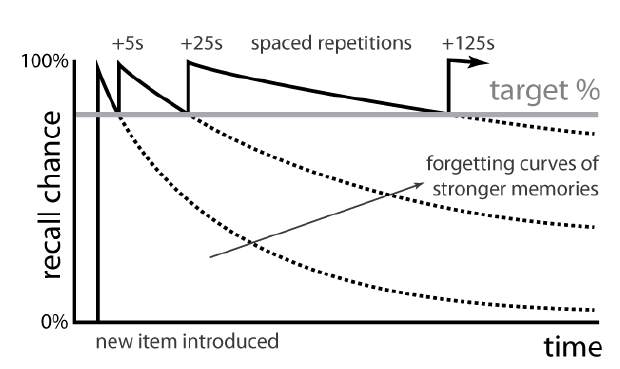
\includegraphics[width=0.5\textwidth]{img/spacedrepetition}
    \caption{Adaptive spaced-repetition learning (taken from \protect\citeA{microlearning})}
    \label{fig:spacedrepetition}
\end{figure}
